\documentclass{beamer}

\makeatletter
\newcommand{\mylabel}{%
   %[\beamer@againname]%
}
\makeatother

\mode<presentation>%
{%
    \usetheme{Rochester}%
    \usecolortheme{beaver}%
}
\setbeamercovered{transparent}
\usepackage{xcolor}
\definecolor{mytransparent}{rgb}{0.8,0.8,0.8}



\usepackage{siunitx}
\usepackage{listings}
\usepackage{graphicx}
\usepackage{subcaption}
\usepackage{amsmath}
\usepackage{hyperref}
\usepackage[backend=bibtex,style=authoryear]{biblatex}
\usepackage[normalem]{ulem}

%%%%%%%%%%%%%%%%% Work flows %%%%%%%%%%%%%%%%%%%%%%%
\usepackage{tikz}
\usetikzlibrary{shapes.geometric,arrows}
\usetikzlibrary{graphs}

\tikzstyle{app} = [rectangle,rounded corners,minimum width=3cm,%
    minimum height = 1cm, text centered, draw =black,fill=red!30]
\tikzstyle{class} = [rectangle,rounded corners,minimum width=2cm,%
    minimum height = .8cm, text centered, draw =black,fill=white]
\tikzstyle{function} = [minimum width=2cm,%
    minimum height = .8cm, text centered, draw =none]
\tikzstyle{arrow}=[thick,->,>=stealth]
\tikzstyle{arrowv}=[thick,dashed,->,>=stealth]


\tikzstyle{startstop} = [rectangle, rounded corners, minimum width=3cm, minimum
height=.5cm,text centered, draw=black, fill=red!30]
\tikzstyle{io} = [trapezium, trapezium left angle=70, trapezium right angle=110,
minimum width=3cm, minimum height=.5cm, text centered, draw=black, fill=blue!30]
\tikzstyle{process} = [rectangle, minimum width=3cm, minimum height=.5cm, text centered, draw=black, fill=orange!30]
\tikzstyle{decision} = [diamond, minimum width=3cm, minimum height=.5cm, text centered, draw=black, fill=green!30]
\tikzstyle{arrow} = [thick,->,>=stealth]
%%%%%%%%%%%%%%%%%%%%%%%%%%%%%%%%%%%%%%%%%%%%%%%%%%%%

\newcommand{\gadget}{\textsc{Gadget-4}}
\newcommand{\grgadget}{\textsc{GrGadget}}
\newcommand{\gramses}{\textsc{GRAMSES}}
\newcommand{\gevolution}{\textsc{Gevolution}}
\newcommand{\pinocchio}{\textsc{Pinocchio}}
\newcommand{\poweri}{\textsc{Poweri4}}
\newcommand{\latfield}{\textsc{LATfield}}
\DeclareMathOperator{\mcm}{mcm}
\DeclareMathOperator{\erfc}{erfc}
\newcommand{\Hconf}{\mathcal{H}}

\title{Relativistic Effects in Cosmological Simulations}
\author{Eduardo Quintana Miranda\\P. Monaco, L. Tornatore}
\date{Trieste 02-05-2023}
\titlegraphic{%
    \includegraphics[height=1cm]{images/logo_oats.png}\hspace*{4cm}~%
    \includegraphics[height=1cm]{images/logo_units.png}%
    }

\bibliography{bibtex.bib}

\begin{document}

\begin{frame}[label=title]
    \titlepage
\end{frame}

\begin{frame}[label=toc]
    \frametitle{Outline\mylabel}
    \tableofcontents
\end{frame}

\section{Introduction}
\frame{\sectionpage}

\begin{frame}[label=cosmologyLCDM]
    \frametitle{The standard cosmological model\mylabel}
    \begin{figure}
        \includegraphics[width=.39\textwidth]{images/dark-sector.png}
        \includegraphics[width=.59\textwidth]{images/planck2015.png}
	\caption{Contents of the universe.
	Planck collaboration 2015.}
    \end{figure}
\end{frame}

\begin{frame}[plain,label=grcosmology]
    \frametitle{Cosmological test of GR\mylabel}
    \begin{figure}
        %\includegraphics[height=.8\textheight]{images/Lensing3D.jpg}
        %\caption{Weak lensing. Credit: NASA/SSU/Aurore Simonnet.}
        \includegraphics[height=.8\textheight]{images/alam-rsd.png}
        \caption{Comparison of RSD. Shadab \emph{et al.} 2020.}
    \end{figure}
\end{frame}

\begin{frame}[plain,label=surveys]
    \frametitle{Surveys\mylabel}
    \begin{figure}
    	\centering
	\begin{subfigure}{0.29\textwidth}
        \includegraphics[width=\textwidth]{images/euclid.jpeg}
	\caption{Euclid satellite.}
	\end{subfigure}
	\hfill
	\begin{subfigure}{0.4\textwidth}
        \includegraphics[width=\textwidth]{images/desi.png}
	\caption{DESI telescope.}
	\end{subfigure}
	\hfill
	\begin{subfigure}{0.39\textwidth}
        \includegraphics[width=\textwidth]{images/lsst.png}
	\caption{Vera Rubin observatory, LSST.}
	\end{subfigure}
    \end{figure}
\end{frame}

\begin{frame}[plain,label=simulations]
    \frametitle{Simulations\mylabel}
    \begin{figure}
        \includegraphics[height=.8\textheight]{images/magneticum.png}
        \caption{Magneticum simulation; Dolag et al. 2015.}
    \end{figure}
\end{frame}

\begin{frame}[label=ligergevolution]
    \frametitle{Relativistic codes\mylabel}
    \begin{figure}
        \centering
        \begin{subfigure}{0.49\textwidth}
        \includegraphics[width=\textwidth,height=.6\textheight]{images/liger-correction.pdf}
        \caption{GR corrections in LIGER$^1$.}
        \end{subfigure}
        \begin{subfigure}{.49\textwidth}
        \includegraphics[width=\textwidth,height=.6\textheight]{images/gevolution-vector-potential.pdf}
        \caption{Gravitomagnetic lines $\nabla\times \vec B$ in
        Gevolution$^2$.}
        \end{subfigure}
    \end{figure}
    \phantom{LIGER\footcite{Bertacca2017}}
    \phantom{GEVOLUTION\footcite{Adamek2016}}
\end{frame}

% \begin{frame}[plain,label=grcosmology2]
%     \frametitle{\mylabel}
%     % TODO results from Bonvin, Lepori, Adamek, Bertaca, Bruni, Durrer, etc
% \end{frame}

\begin{frame}[label=pmvstreepm]
    \frametitle{TreePM vs PM\mylabel}
    \begin{figure}
        \begin{subfigure}[b]{.49\textwidth}
        \includegraphics[width=\textwidth]{images/gevolution-z0.png}%
        \caption{\gevolution\ (PM)}
        \end{subfigure}
        \begin{subfigure}[b]{.49\textwidth}
        \includegraphics[width=\textwidth]{images/gadget-z0.png}%
        \caption{\gadget\ (TreePM)}
        \end{subfigure}
    \end{figure}
\end{frame}


\section{Relativistic effects}
\frame{\sectionpage}


\begin{frame}[label=metric]
    \frametitle{Metric and gauge\mylabel}
   \newcommand{\qq}{p^2+m^2 a^2}
    In the weak field limit we can treat the gravity of $N$-bodies 
    as a perturbation of the FLRW metric:
    \begin{equation}
    \begin{split}
        ds^2
        &= g_{\mu\nu} dx^{\mu}dx^{\nu} = (\hat g_{\mu\nu} + \delta
        g_{\mu\nu})dx^{\mu} dx^{\nu} \\
        &= a^2 \big( 
            - (1+2\Psi)d\tau^2
            - 2 B_i dx^i d\tau
             + ((1-2\Phi) \delta_{ij}+ h_{ij}) dx^i dx^j \big) \\
    \end{split}
    \end{equation}
    in the Poisson gauge we have
    \[
        B^i{}_{,i} =  h^{i}{}_i =  h^i{}_{j,i} = 0
    \]
    we usually use $\chi=\Phi-\Psi$.
\end{frame}

\begin{frame}{label=fieldeq}
    \frametitle{Field equations}%
    From Einstein equations we obtain
    \begin{equation}
        \nabla^2 \Phi 
        - 3\frac{\Hconf}{c^2} \dot\Phi -
        3\frac{\Hconf^2}{c^2} \Phi
        = \frac{4\pi G a^2}{c^4} \Delta T^0{}_0
    \end{equation}
    \begin{equation}
        \nabla^2 B_i
        = \frac{16\pi G a^2}{c^4} \Delta T^0{}_i - 4\partial_i(
        \frac{\dot\Phi}{c} +
        \frac{\Hconf}{c} \Psi  )
    \end{equation}
    \begin{equation}
        \nabla^2 \chi
        = \frac{4\pi G a^2}{c^4} \Delta T^n{}_n + 3 \frac{\Hconf^2}{c^2} \Phi
    \end{equation}
    \begin{equation}
        \frac{1}{c^2} \ddot h^i{}_j- \nabla^2 h^i{}_j + 2 \frac{\Hconf}{c^2} {\dot h}^i{}_j
        = - \frac{16\pi G a^2}{c^4} P_{\perp}\left( \Delta T^i{}_j -
	\frac{\delta^i_j}{3} \Delta T^n{}_n\right)
    \end{equation}
\end{frame}

\begin{frame}[label=greffects]
    \frametitle{Relativistic effects\mylabel}
    \begin{itemize}
        % see yoo-0907.0707 and liger-1703.03407
        \item redshift space distortions: doppler, Sachs-Wolf and ISW.
        % redshift space distortion due to peculiar velocities
        % of the source and observer, potential
        % well of the scalar of the metric and frame-dragging + the integrated
        % effect along the line of sight.
        \[
            \frac{\delta z}{z}
            =  [ (v_i - B_i) e^i - \Psi ]^s_{o} - \int_o^{r_s} dr
            [\dot\Phi+\dot\Psi -
            B_{i|j} e^i e^j]
        \]
        \item number counts
        % deflection of the photon, translates into a displacement of the observed
        % position of the source on the sky, and magnification
        \[
            \Delta (\vec n, z) = 
            \Delta_{\mathrm{dens}}
            + \Delta_{\mathrm{rsd}}  % RSD
            + \Delta_{\kappa}        % weak lensing convergence
            + \Delta_{\mathrm{gr}}   % general relativistic
        \]
    \end{itemize}
\end{frame}


\section{GrGadget, Code design and algorithms}
\frame{\sectionpage}

\begin{frame}[label=octtreepm]
    \frametitle{GrGadget: a TreePM relativistic N-body code\mylabel}
    \begin{columns}
        \begin{column}{.5\textwidth}
	\vspace*{\fill}
            \begin{figure}
                \includegraphics[height=.5\textheight]{images/octree.png}
                \caption{\gadget.}
            \end{figure}
        \end{column}
        \begin{column}{.5\textwidth}
	\vspace*{\fill}
            \begin{figure}
                \includegraphics[height=.5\textheight]{images/cubic-grid.jpeg}
                \caption{\gevolution.}
            \end{figure}
        \end{column}
    \end{columns}
\end{frame}

\begin{frame}[plain,label=pmchart]
    \vspace*{-.5cm}
     \begin{figure}
         \begin{subfigure}[b]{.48\textwidth}
             \caption{Newtonian PM}
             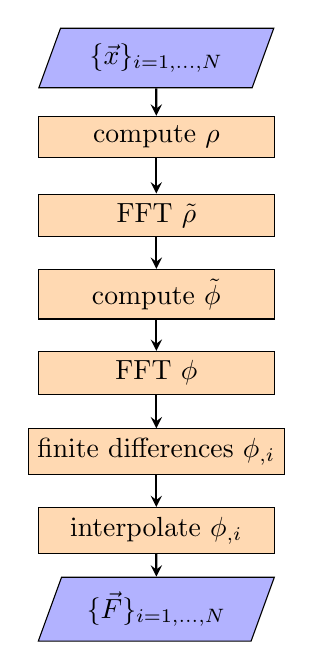
\begin{tikzpicture}[node distance=1cm]
                 \node (in) [io] {\{$\vec x\}_{i=1,\ldots,N}$};
                 \node (f1) [process, below of=in] {compute $\rho$};
                 \node (f2) [process, below of=f1] {FFT $\tilde\rho$};
                 \node (f3) [process, below of=f2] {compute $\tilde\phi$};
                 \node (f4) [process, below of=f3] {FFT $\phi$};
                 \node (f5) [process, below of=f4] {finite differences $\phi_{,i}$};
                 \node (f6) [process, below of=f5] {interpolate $\phi_{,i}$};
                 \node (out) [io, below of=f6] {\{$\vec F\}_{i=1,\ldots,N}$};
                 \draw [arrow] (in) -- (f1);
                 \draw [arrow] (f1) -- (f2);
                 \draw [arrow] (f2) -- (f3);
                 \draw [arrow] (f3) -- (f4);
                 \draw [arrow] (f4) -- (f5);
                 \draw [arrow] (f5) -- (f6);
                 \draw [arrow] (f6) -- (out);
             \end{tikzpicture}        
         \end{subfigure}
         \hfill
         \begin{subfigure}[b]{.48\textwidth}
             \caption{Relativistic PM}
             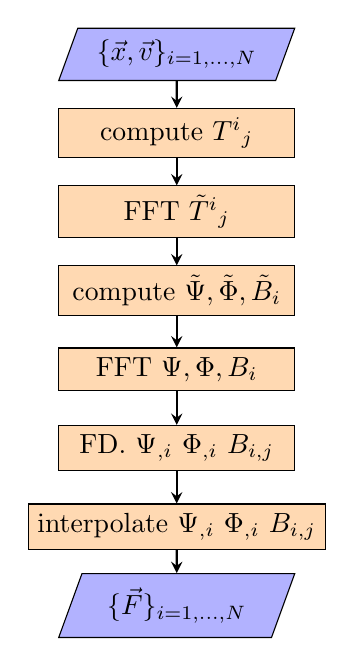
\begin{tikzpicture}[node distance=1cm]
                 \node (in) [io] {\{$\vec x, \vec v\}_{i=1,\ldots,N}$};
                 \node (f1) [process, below of=in] {compute $T^i{}_j$};
                 \node (f2) [process, below of=f1] {FFT $\tilde T^i{}_j$};
                 \node (f3) [process, below of=f2] {compute $\tilde \Psi,\tilde
                 \Phi, \tilde B_i$};
                 \node (f4) [process, below of=f3] {FFT $\Psi,\Phi,B_i$};
                 \node (f5) [process, below of=f4] {%
                     FD. $\Psi_{,i}$ $\Phi_{,i}$ $B_{i,j}$};
                 \node (f6) [process, below of=f5] {%
                     interpolate
                     $\Psi_{,i}$ $\Phi_{,i}$ $B_{i,j}$};
                 \node (out) [io, below of=f6] {\{$\vec F\}_{i=1,\ldots,N}$};
                 \draw [arrow] (in) -- (f1);
                 \draw [arrow] (f1) -- (f2);
                 \draw [arrow] (f2) -- (f3);
                 \draw [arrow] (f3) -- (f4);
                 \draw [arrow] (f4) -- (f5);
                 \draw [arrow] (f5) -- (f6);
                 \draw [arrow] (f6) -- (out);
             \end{tikzpicture}        
         \end{subfigure}
     \end{figure}
\end{frame}

\begin{frame}[label=challenges]
    \frametitle{Technical challenges\mylabel}
    \begin{itemize}
    	\setlength\itemsep{1em}
    	\item Code re-engineering;
		% memory layout, context, unit conversion, MPI coordination
	\item Domain decomposition;
	\item Drift operator;
	\item TreePM force addition;
    \end{itemize}
\end{frame}

\begin{frame}[label=codedesign]
    \frametitle{GrGadget\mylabel}
    \begin{figure}
        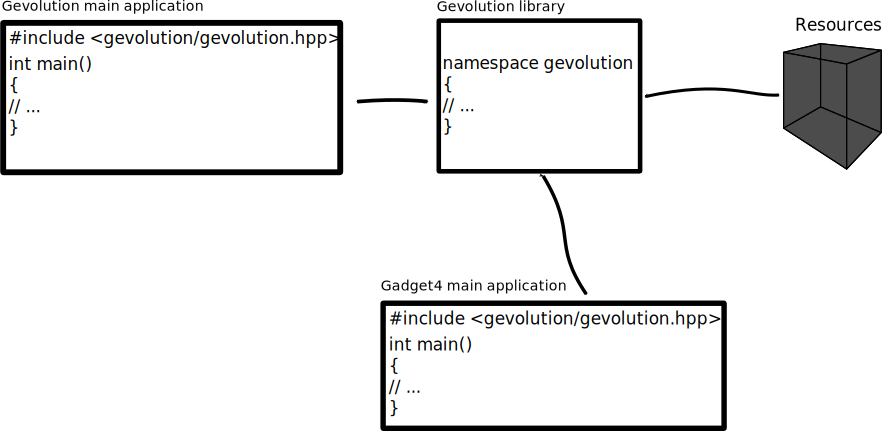
\includegraphics[width=\textwidth]{images/modular-code.png}
    \end{figure}
\end{frame}
% \begin{frame}[label=memorylayout]
%     \frametitle{GrGadget developement\mylabel}
%     % fig. 2 of the code paper, ownership and relations
%     \vspace*{-.5cm}
%     \begin{figure}
%     \centering\includegraphics[width=\textwidth]{%
%         images/base_pm.pdf}%
%         \caption{Resource ownership in GrGadget.}
%     \end{figure}
% \end{frame}




\begin{frame}[label=meshdomains]
    \frametitle{Domain decomposition\mylabel}
    \begin{figure}
        \centering
        \includegraphics[width=.8\textwidth]{images/domains.png}
    \end{figure}
\end{frame}

\begin{frame}[label=drift1]
    \frametitle{Adjustment to Gadget's drift\mylabel}
\begin{columns}
    \begin{column}{0.5\textwidth}
    \begin{figure}
        \centering
        \includegraphics[height=.8\textheight]{images/leap-frog.png}
        \caption{Gadget's leap-frog integration.}
    \end{figure}
    \end{column}
    \begin{column}{0.5\textwidth}
    The particle data structure has:
    \begin{itemize}
        \item $\vec x$
        \item $\vec p/m$ (momentum per unit mass)
        \item $\Phi$, $\vec B$
    \end{itemize}
    then the drift is done as
    \[
        \Delta x^i
        = \frac{\Delta\tau}{a}((1+3\Phi)p^i/m + c B^i a )
    \]
    the kicks change $\vec p/m$.
    \end{column}
\end{columns}
\end{frame}

% \begin{frame}[label=drift2]
%     \frametitle{Time steps\mylabel}
%     \begin{figure}
%         \includegraphics[width=\textwidth]{images/gadget4-timestep.png}
%     \end{figure}
% \end{frame}



\begin{frame}[label=forceaddition1]
    \frametitle{Tree and PM coupling\mylabel}
\begin{align*}
    \tilde\phi_k 
    &= -\frac{4\pi}{k^2} \tilde\rho_k \\
    &= -\frac{4\pi}{k^2} \tilde\rho_k \left( 1 - \exp(-k^2 r_a^2) \right)
       -\frac{4\pi}{k^2} \tilde\rho_k \exp(-k^2 r_a^2)
\end{align*}
the long range potential $\tilde\phi^{(\mathcal{L})}_k$ is computed in the PM
\[
    \tilde\phi^{(\mathcal{L})}_k
    = -\frac{4\pi}{k^2} \tilde\rho_k \exp(-k^2 r_a^2)
\]
and the short range potential $\phi^{(s)}$ is computed by the Tree
\[
    \phi^{(\mathcal{S})}(\vec x)
    = \sum_i - \frac{m_i G}{|\vec x - \vec x_i|} 
        \erfc\left(\frac{|\vec x-\vec x_i|}{2 r_a}\right)
\]
$r_a$ is the PM smoothing scale.
\end{frame}

\begin{frame}[label=forceaddition2]
    \frametitle{TreePM force correction\mylabel}
    % TreePM force addition
let $\color{red} r_b$ be the GR smoothing scale and $\color{blue}r_a$ the PM smoothing scale:
\[
    F^{\text{TreePM}}
    =
    {\color{red} 
       \mathcal{L}[F_{\text{GR}}^{\text{PM}}-F_{\text{Newton}}^{\text{PM}}]
    }
    +{\color{blue}\mathcal{L}[F_{\text{Newton}}^{\text{PM}}]
    +\mathcal{S}[F_{\text{Newton}}^{\text{Tree}}]}
\]
    
    \begin{columns}
    \begin{column}{0.5\textwidth}
        in the large scales $k\ll N/L$
        \begin{itemize}
            \item 
                ${\color{red} \mathcal{L} [ F_{\text{GR}}^{\text{PM}} ] }=F_{\text{GR}}$
            \item
                ${\color{red} \mathcal{L} [ F_{\text{Newton}}^{\text{PM}} ] }=F_{\text{Newton}}$
            \item
            ${\color{blue}\mathcal{L}[F_{\text{Newton}}^{\text{PM}}]}=F_{\text{Newton}}$,
            \item
            ${\color{blue}\mathcal{S}[F_{\text{Newton}}^{\text{Tree}}]}=0$, 
        \end{itemize}
    \end{column}
    \begin{column}{0.5\textwidth}
        on small scales $k\gg N/L$
        \begin{itemize}
            \item 
                ${\color{red} \mathcal{L}[ 
                    F_{\text{GR}}^{\text{PM}} 
                    -F_{\text{Newton}}^{\text{PM}} 
                    ] } = 0$
            \item 
            ${\color{blue}\mathcal{L}[F_{\text{Newton}}^{\text{PM}}]}=0$,
            \item
            ${\color{blue}\mathcal{S}[F_{\text{Newton}}^{\text{Tree}}]}
                =F_{\text{Newton}}$, 
        \end{itemize}
    \end{column}
    \end{columns}
\end{frame}

\section{Tests and Results}
\frame{\sectionpage}

% \begin{frame}[label=testsummary]
%     \frametitle{\mylabel}
%     \begin{itemize}
%     	\setlength\itemsep{1em}
%     	\item Newtonian forces; 
% 		% sanity check, coherent Tree+PM addition
% 	\item Matter power spectrum, in Newtonian regime;
% 		% expect near identical amplitudes
% 	\item GR matter power spectrum; 
% 		% expect matching in the small scales and GR features in the
% 		% large scales
% 	\item Potentials power spectrum;
% 		% TreePM vs PM,
% 	\item GR smoothing scale;
% 		% what are the results of diffent rb choices?
% 		% how far can we extend the GR limit?
% 	\item Convergence/resolution test;
% 		% do we get the same results when we change the resolution of
% 		% the simulations?
% 	\item Performance of the code;
% 		% What is the comp. burden of running GrGadget with a GR PM
% 		% instead of the Newtonian PM?
%     \end{itemize}
% \end{frame}

\begin{frame}[label=forcetest]
    \frametitle{Newtonian force test\mylabel}
    \vspace*{-.5cm}
    \begin{columns}
        \begin{column}{.65\textwidth}
            \centering\includegraphics[width=\textwidth]{%
                images/forcetest/dist-relation.png} 
        \end{column}
        \begin{column}{.35\textwidth}
            \begin{itemize}
               \item $N = 256$ grid size
               \item $L = \SI{1}{Gpc}/h$
            \end{itemize}
        \end{column}
    \end{columns}
    {\small Forces due to a point source. RMS of the difference between real and
    TreePM forces.}
\end{frame}

\begin{frame}[label=forcetest2]
    \frametitle{Newtonian force test\mylabel}
    \vspace*{-.5cm}
    \begin{columns}
        \begin{column}{.65\textwidth}
            \only<1>{\centering\includegraphics[width=\textwidth]{%
                images/forcetest/gadget-gev-pm-diff-z8-64.pdf}}%
            \only<2>{\centering\includegraphics[width=\textwidth]{%
                images/forcetest/gadget-gev-pm-diff-z0-64.pdf}}%
        \end{column}
        \begin{column}{.35\textwidth}
            \begin{itemize}
               \only<1>{\item $z=8$}
               \only<2>{\item $z=0$}
               \item $N_p = 64^3$ particles
               \item $N = 64$ grid size
               \item $L = \SI{1}{Gpc}/h$
            \end{itemize}
        \end{column}
    \end{columns}
    \small A dark matter-only \gadget\ simulation. Newtonian force dispersion
    due to numerical approximations.\footnote{Forces are given Gadget units
    $(\text{km/s})^2\, h/\text{kpc}$.}
\end{frame}

\begin{frame}[label=matterpower]
    \frametitle{Matter power spectrum\mylabel}
    \vspace*{-.5cm}
    \begin{figure}
    \centering\includegraphics[height=.8\textheight]{%
        images/gad-gev-first-power/pw-008.pdf}%
        \caption{Matter power spectrum. $N=256^3$, $L=\SI{1}{Gpc}/h$.}
    \end{figure}
\end{frame}

\begin{frame}[label=matterpower2]
    \frametitle{Matter power spectrum\mylabel}
    \vspace*{-.5cm}
    \begin{figure}
    \centering\includegraphics[height=.8\textheight]{%
        images/gad-gev-latest-power/pw-008.pdf}%
        \caption{Matter power spectrum. $N=512^3$, $L=\SI{500}{Mpc}/h$.}
    \end{figure}
\end{frame}

\begin{frame}[label=matterpowerGR]
    \frametitle{Matter power spectrum\mylabel}
    \vspace*{-.5cm}
    \begin{figure}
    \centering\includegraphics[height=.8\textheight]{%
        images/gad-gev-gr-power/pw-008.pdf}%
        \caption{Matter power spectrum. $N=512^3$, $L=\SI{500}{Mpc}/h$.}
    \end{figure}
\end{frame}


\begin{frame}[label=Phipower]
    \frametitle{Potentials power spectrum\mylabel}
    % testing the fields power spectrum
    % 1. probably the most important feature of our code
    %    - relativistic potentials at non-linear scales are better resolved
    %    thanks to the realistic matter distribution.
    %    - for instance see Phi
    %\[
    %    ds^2 = a^2( -(1+2\Psi)d\tau^2 - 2 B_i d\tau dx^i+ (1-2\Phi)\gamma_{ij} dx^i dx^j)
    %\]
    \vspace*{-.5cm}
    \begin{figure}
    \only<1>{\centering\includegraphics[height=.8\textheight]{%
        images/pw-phi.pdf}}%
    \only<2>{\centering\includegraphics[height=.8\textheight]{%
        images/pw-phi-plus.pdf}}%
        \caption{$\Phi$ power spectrum. $N=256^3$ $L=\SI{1}{Gpc}/h$.}
    \end{figure}
\end{frame}

\begin{frame}[label=Bipower]
    \frametitle{Potentials power spectrum\mylabel}
  \def\path{images}%
  \begin{figure}
      \begin{subfigure}[t]{.49\textwidth}
      \includegraphics[width=\textwidth]{\path/pw-Bi.pdf}%
      \caption{$B_i$ single component power spectrum.}
      \end{subfigure}
      \begin{subfigure}[t]{.49\textwidth}
      \includegraphics[width=\textwidth]{\path/pw-chi.pdf}%
      \caption{$\chi$ power spectrum.}
      \end{subfigure}
  \end{figure}
\end{frame}

\begin{frame}[label=grcuttest]
    \frametitle{Gr smoothing scale\mylabel}
  \def\path{images/test-gr-cut}%
  \begin{figure}
      \includegraphics[height=\textheight]{\path/high-res-006.pdf}%
  \end{figure}
\end{frame}

\begin{frame}[plain,label=resolutiontest]
    \vspace*{-.8cm}
  \centering\includegraphics[height=1.4\textheight]{images/resolution.pdf}
\end{frame}


\begin{frame}[label=performancetime]
   \frametitle{Performance\mylabel}
  \vspace*{-.5cm}
  \begin{figure}
      \includegraphics[height=.8\textheight]{images/appendix/gr-vs-newton.pdf}%
      \caption{Timing of Gevolution's PM in Gadget, respect to total runtime.
      $L$ goes from $250$ to $\SI{2000}{Gpc}/h$.}
  \end{figure}
\end{frame}

\begin{frame}[label=performancescaling]
 \frametitle{Performance\mylabel}
  \vspace*{-.5cm}
  \begin{figure}
      \begin{subfigure}[b]{.49\textwidth}
      \includegraphics[width=\textwidth]{images/appendix/strong-scale-Total.pdf}%
      \caption{Strong scalability.}
      \end{subfigure}
      \begin{subfigure}[b]{.49\textwidth}
      \includegraphics[width=\textwidth]{images/appendix/weak-scale-Total.pdf}%
      \caption{Weak scalability.}
      \end{subfigure}
  \end{figure}
\end{frame}

\section{Concluding remarks}
\frame{\sectionpage}

\begin{frame}[label=conclusions]
    \frametitle{\insertsection\mylabel}
    \begin{itemize}
    	\item We have constructed a relativistic TreePM code, \grgadget
	(Quintana-Miranda, Monaco, Tornatore. MNRAS 2023);
	\item \grgadget\ is able to extract relativistic effects from high
	resolution matter realizations;
	\item We estimate our assumptions are valid for
	$3L/N \le r_b \le \SI{6}{Mpc}/h$;
    \end{itemize}
    \begin{block}{}
	    \url{https://github.com/GrGadget}
    \end{block}
\end{frame}

\begin{frame}[label=outlook]
    \frametitle{Outlook\mylabel}
    \begin{equation}
        \nabla^2 B_i
        = \frac{16\pi G a^2}{c^4} \Delta T^0{}_i - 4\partial_i(
        \frac{\dot\Phi}{c} +
        \frac{\Hconf}{c} \Psi  )
    \end{equation}
    The presence of vector perturbations will be detectable in the RSD
    multipoles at $x<\SI{10}{Mpc}/h$ (Bonvin et al. 2018).
    % either as a test for GR over mod. gravity
    % or as an additional effect to consider to avoid systematic errors.
    
    \vskip1em
    
    Vorticity is enhanced by velocity dispersion in f(R) theories (Thomas et al.
    2015).
    
    \vskip1em
    
    We could use GrGadget to extract the unique GR or mod. gravity signals from
    RSD.
    
\end{frame}

\begin{frame}[label=questions]
    \frametitle{Questions}
\end{frame}

\begin{frame}[label=forcesnpotentials]
    \frametitle{from potentials to forces\mylabel}
    finite differences is used to derive potentials in order to compute the
    forces.
    first order:
    \[
        \frac{\partial \Phi_i}{\partial x} = \frac{ \Phi_{i+1} - \Phi_i }{h} + O(h)
    \]
    second order:
    \[
        \frac{\partial \Phi_i}{\partial x} =
         \frac{ \Phi_{i+1} - \Phi_{i-1} }{2h} + O(h^2)
    \]
    next order:
    \[
        \frac{\partial \Phi_i}{\partial x} =
        8\frac{ \Phi_{i+1} - \Phi_{i-1} }{12h} 
            - \frac{ \Phi_{i+2} - \Phi_{i-2} }{12h} + O(h^4)
    \]
\end{frame}

\begin{frame}[label=differencesPM]
	\frametitle{Differences between \gadget\ and \gevolution\mylabel}
	\begin{tabular}{ccc}
		& \gadget\ & \gevolution \\
		\hline
		Sampling/Interpolation corrections & Yes & No \\
		Finite differences & $O(h^4)$ & $O(h)$ \\
		Laplace operator ($\nabla^2$) & $-k^2 $
			& $- \frac{4 N^2}{L^2}\sin^2 \left(\frac{k L}{2N}\right) $\\
	\end{tabular}
\end{frame}

\end{document}
%%%%%%%%%%%%%%%%%%%%%%%%%%%%%%%%%%%%%%%%%%%%%%%%%%%%%%%%%%%%%%%%%%%%%%%%%%%%%%%%%%%

\begin{frame}[label=geodesics]
    \frametitle{Geodesics}
    % B plays the role of a vector potential, like in Electrodynamics.
    in the limit of $p\ll ma$ (small velocities) and using physical time
   \newcommand{\qq}{p^2+m^2 a^2}
    $dt = a d\tau$ we obtain 
    \begin{equation}
        \frac{d^2\vec x}{dt^2}
        = -2H \frac{d\vec x}{dt} 
          - \frac{1}{a^2}\vec\nabla \Phi
          + \frac{1}{a}(H + \partial_t)\vec B
          - \frac{1}{a} \frac{d\vec x}{dt}\times (\vec\nabla\times\vec B)
    \end{equation}
\end{frame}
\begin{frame}{label=fieldeq}
    \frametitle{Field equations}%
    $\Phi$ is sourced by $\Delta T^0{}_0$
    \begin{equation}
        \nabla^2 \Phi 
        - 3\frac{\Hconf}{c^2} \dot\Phi -
        3\frac{\Hconf^2}{c^2} \Phi
        = \frac{4\pi G a^2}{c^4} \Delta T^0{}_0
    \end{equation}
    $B_i$ is sourced by the transversal component of $\Delta T^0{}_i$
    % that is, in the gauge we have fixed, B is divergenless. The divergenless
    % part of that equations sources B, while the other component sources a
    % combination of the potentials.
    \begin{equation}
        \nabla^2 B_i
        = \frac{16\pi G a^2}{c^4} \Delta T^0{}_i - 4\partial_i(
        \frac{\dot\Phi}{c} +
        \frac{\Hconf}{c} \Psi  )
    \end{equation}
    $\chi = \Phi-\Psi$ is sourced by $\Delta T^n{}_n$
    \begin{equation}
        \nabla^2 \chi
        = \frac{4\pi G a^2}{c^4} \Delta T^n{}_n + 3 \frac{\Hconf^2}{c^2} \Phi
    \end{equation}
\end{frame}


\begin{frame}[label=libgevolutioninheritance]
    \frametitle{Libgevolution: Design and concepts}
    % The concept we are abtracting here is a parallel-PM.
    % Then that concept can be specialized on whether the physics follows a
    % Newtonian prescription or a relativistic one, or mod grav.
    % The implementation details are hidden behind this abstraction layer,
    % so now we use Fourier Methods, we might as well in the future use
    % and adaptive mesh but the API SHOULDNT change.
\begin{figure}
    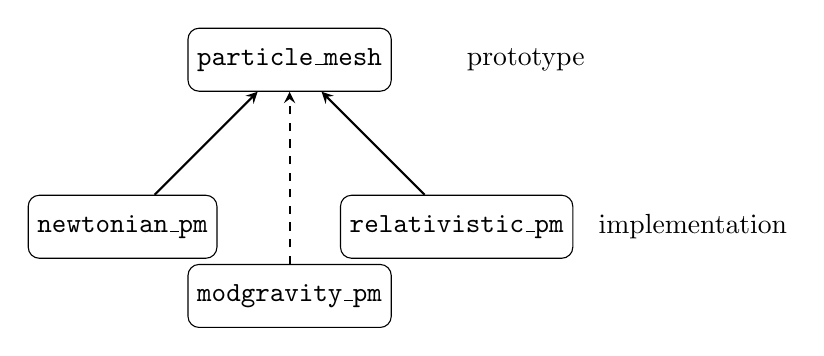
\begin{tikzpicture}[node distance=3cm]
        \node (pm) [class] {\texttt{particle\_mesh}};
        \node (newton) [class, below left of=pm]{\texttt{newtonian\_pm}};
        \node (gr) [class, below right of=pm]{\texttt{relativistic\_pm}};
        \node (modgr) [class, below of=pm]{\texttt{modgravity\_pm}};
        \draw [arrow] (gr) -- (pm);
        \draw [arrow] (newton) -- (pm);
        \draw [arrow,dashed](modgr) -- (pm);
        \node (com1) [right of=pm] {prototype};
        \node (com2) [right of=gr] {implementation};
    \end{tikzpicture}
    \caption{PM class: it does particle-mesh stuff.}
\end{figure}
\end{frame}


\begin{frame}[label=applications]
    \frametitle{Possible applications:}
    \begin{itemize}
        \item contrain modified gravity models with observables,
        for example the distortion parameter
        characterizing RSD.
    \end{itemize}
    \begin{figure}
        \centering\includegraphics[width=\textwidth]{images/alam-2020.png}
        \caption{Multipoles of the RSD. Alam et al \texttt{arxiv:2011.05771}}
    \end{figure}
\end{frame}
